\documentclass[12pt]{article}

\usepackage[spanish]{babel}
\usepackage{hyperref}
\usepackage{graphicx}
\usepackage{listings}
\usepackage{color}
\usepackage{multicol}
\usepackage{amssymb}
\usepackage{enumitem}
\usepackage{here}
\usepackage{dsfont}
\usepackage{amsmath}
\spanishdecimal{.}

\title{Matemáticas para las Ciencias Aplicadas I}
\title{
	Segunda Lista de Problemas \\
	\textbf{Segunda Parte} \\
	\vspace{1ex}
	\large Matemáticas para las Ciencias Aplicadas I \\
	Facultad de Ciencias, UNAM}

\date{\today}

\author{Flores Morán Julieta Melina \\ Zarco Romero José Antonio}

\begin{document}

\maketitle

%% 5, 10, 20, 36 y 40

%% 1
\section{Ejercicio 5} 
Utilice una aproximación cuadrática local apropiada para aproximar $\tan 61^{\circ}$ y compare el resultado con el producido directamente por su utilidad de cálculo.

%% 2
\section{Ejercicio 10}
\[\sin \pi x\]

Encuentre los polinomios de Maclaurin de orden $n = 0, 1, 2, 3, 4$, y luego encuentre los polinomios de Maclaurin enésimos para la función en notación sigma.

%% 3
\section{Ejercicio 20}
\[\frac{1}{x+2}\text{; }x_0=3\]

Encuentre los polinomios de Taylor de orden $n = 0, 1, 2, 3, 4$ alrededor de $x = x_0$ y luego encuentre el enésimo polinomio de Taylor para la función en notación sigma.

%% 4
\section{Ejercicio 36}
\[\frac{1}{e}\text{; precisión de tres decimales}\]

Utilice el método del ejemplo 7 para aproximar la expresión dada a la precisión especificada. Verifique su respuesta con la producida directamente por su utilidad de cálculo.

%% 5
\section{Ejercicio 40}
\begin{figure}[h!]
\centering
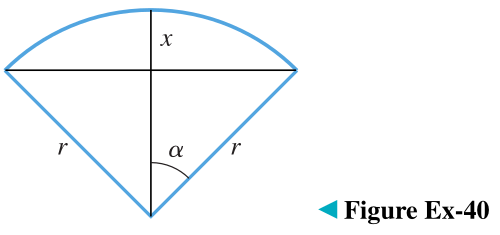
\includegraphics[width=0.5\textwidth]{../img/img_Lista2/2_40.png}
\end{figure}
\begin{enumerate}[label=(\alph*)]
\item La figura adjunta muestra un sector de radio $r$ y ángulo central $2 \alpha$. Suponiendo que el ángulo $\alpha$ es pequeño, utilice la aproximación cuadrática local de $\cos \alpha$ en $\alpha = 0$ para demostrar que $x \approx r \alpha ^2/2$.
\item Suponiendo que la Tierra es una esfera de radio $4000 mi$, use el resultado del inciso $(a)$ para aproximar la cantidad máxima en la que un arco de $100 mi$ a lo largo del ecuador divergirá de su cuerda.
\end{enumerate}

\end{document}
